\documentclass[xcolor=dvipsnames]{beamer}

\usepackage[utf8]{inputenc}
\usepackage[francais]{babel}
\usepackage{verbatim}
\setcounter{tocdepth}{1}

%\usecolortheme[named=purple]{structure}
\usecolortheme[named=brown]{structure}
\usetheme{Hannover}
%\useitemizeitemtemplate{\small\raise1.5pt\hbox{\donotcoloroutermaths$\heartsuit$}}
%\usesubitemizeitemtemplate{\scriptsize\raise1.5pt\hbox{\donotcoloroutermaths$\heartsuit$}}
%\usesubsubitemizeitemtemplate{\tiny\raise1.5pt\hbox{\donotcoloroutermaths$\heartsuit$}}
\useitemizeitemtemplate{\scriptsize\raise1.5pt\hbox{\donotcoloroutermaths$\blacktriangleright$}}
\usesubitemizeitemtemplate{\tiny\raise1.5pt\hbox{\donotcoloroutermaths$\rhd$}}

\title{\textsc{Lil'Bro}\\\tiny\textit{watching everything, everywhere}}
\author{Groupe d'étude H4213}
%\author{H4213\\ Fabrice Gabolde --- Guillaume Bouchard\\Guillaume Ayoub --- Nicolas Kandel\\Pierre-Yves David --- Rémi Thévenoux}

\begin{document}

\frame{\titlepage}
\frame{\tableofcontents}



%6 intervenants




%Yabs parle de l'architecture generale + du coup du partenariat pour les antennes GSM
\section{Architecture}

\frame{
\frametitle{Architecture générale de l'application}
\begin{figure}[h!]
\centering
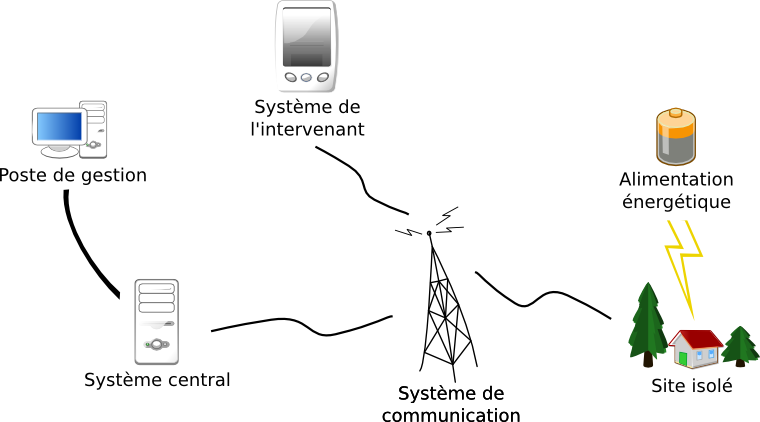
\includegraphics[width=\textwidth]{schema_architecture_generale.png}
%\caption{Schéma de l'architecture générale}
\end{figure}
}


\section{Communication}

\frame{
\frametitle{Modes de communication}

\begin{itemize}
\item Technologies éprouvées (GPS, Internet, USB, etc.)
\item Partenariat avec des opérateurs locaux
\end{itemize}
}

%Nicolas fait la promo du PDA pour l'intervenant sur site

\section{Intervenant}

\frame{
\frametitle{Dispositifs de l'intervenant}


\begin{itemize}
\item Interfaces simplifiées
\item Géolocalisation
\item Informations en temps réel
\end{itemize}

}

\section{Système central}

%Remi parle du systeme distant et du serveur

\frame{
\frametitle{Système central}

\begin{itemize}
\item Multiples services
\item Multiples clients possibles
\end{itemize}

}


% Marmoute

\section{Système distant}

\frame{
\frametitle{Système distant}

\begin{itemize}
\item Autonomie
\item Fiabilité
\item Technologie éprouvée
\end{itemize}

}


%Mikado peut parler des procedures mises en place pour assurer la qualité
\section{Qualité}


\frame{
\frametitle{Qualité}

\begin{itemize}
\item Outils de suivi des documents
\item Critères de qualité sur les achats
\item Vue d'ensemble pour l'homogénéité
\end{itemize}

}


% conclusion
\section{Conclusion}

\frame{
\frametitle{Conclusion}

\begin{itemize}
\item Plus grande réactivité en termes de maintenance
\item Contrôle à distance
\item Modularité et adaptabilité
\item Technologies éprouvées
\item Coûts réduits
\end{itemize}

\textit{La réunion des meilleures technologies en vue de la réussite}
}
\end{document}

% Exemple de page
% \frame{
% \frametitle{blu}
% Scénario :
% \begin{itemize}
% \item bite,
% \item cul.
% \end{itemize}
% }

% Schéma
% \frame{
% \frametitle{Architecture générale de l'application}
% \begin{figure}[h!]
% \centering
% 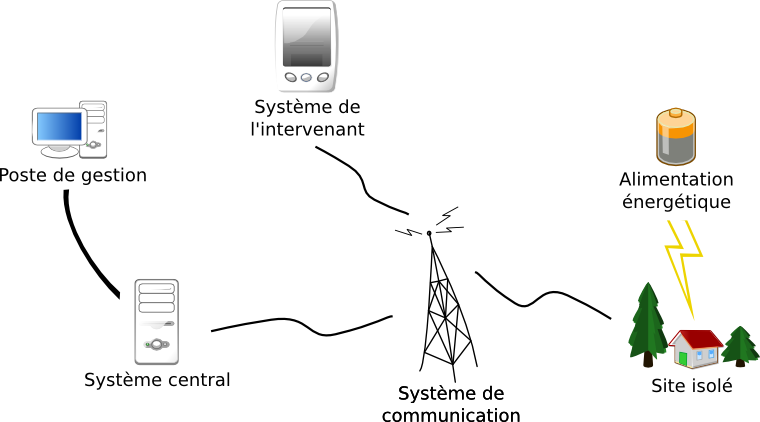
\includegraphics[width=\textwidth]{schema_architecture_generale.png}
% \caption{Schema de l'architecture générale}
% \end{figure}
% }
